%Chapter 1

\renewcommand{\thechapter}{1}

\chapter{The State of the Art}

\section{Resilience Definitions}


\subsection{Mechanical Engineering}
Mechanical Engineering has a very specific definition of resilience as
a characteristic of a material. Resilience is the ability of a
material ``to store or absorb energy without permanent deformation''
\cite{Popov1964}.
The modulus of resilience is a property used to compare
materials for use in applications where energy must be absorbed by the
component without permanently altering the component's geometry. When
the plastic deformation is taken into account, the area under the
stress strain curve until fracture is a material's toughness. Both of
these concepts have use in our exploration. As we will see, the
modulus of resilience is analogous to engineering resilience
\cite{Holling1973a}
while toughness is analogous to ecological resilience.

\subsection{Ecology}
The field of ecology has a rich history with resilience, and many
concepts and applications may be portable to the engineering domain,
especially when considering complex systems' resilience such as
infrastructure resilience, community resilience, and System of Systems
(SoS) resilience. Multiple papers have laid out the history of this
thinking, and the resilience mindset is a common discussion item by
practitioners and leading researchers in the field \cite{Curtin2014}.
explore the history of resilience-thinking in ecology. The
narrative progresses from introductory concepts of resilience through
more complex iterations including panarchy, and finally prospects for
action in adaptive management. Holling first introduced resilience to ecology in his
seminal work Resilience and Stability of Ecological Systems
\cite{Holling1973a} where heproposed two types of resilience: engineering
resilience and ecological resilience.

\subsubsection{Engineering Resilience}
Engineering resilience is a system's ability to return to status quo
performance \cite{Holling2010}. Engineering resilience is similar to
the mechanical engineering concept of modulus of resilience because
both concepts describe behavior against a status quo prior to the
changing force.

\subsubsection{Ecological Resilience}
Ecological resilience is a system's ability to persist through input
changes and to establish different equilibria after a disturbance. The
equilibria may be called basins of attraction in the ecological
literature. The terminology, basins of attraction, better describes
the system behavior of socio-ecological systems. The relationship
between entities in the system, such as predator and prey populations,
are not steady equilibria. The values cycle about the domain of
attraction. A system may have multiple basins of attraction. When a
disturbance changes the inputs to the system, the system undergoes
regime change, and the trajectory of the system in its state space
transitions around a new basin of attraction \cite{Folke2010a}. While
more complex, this definition of resilience shares similarities to the
definition of toughness because both concepts describe system
persistence through disturbance while accumulating changes to its
composition.

\subsection{Risk Analysis}
The Society of Risk Analysis has defined resilience with a family of
definitions \cite{Aven2015b}:
\begin{quotation}
  \begin{itemize}
    \item Resilience is the ability of the system to sustain or
      restore its basic functionality following a risk source or an
      event (event unknown).
    \item Resilience is the sustainment of the system's operations
      and associated uncertainties, following a risk source or an
      event (event unknown).
    \item Resilience is the ability of a system to reduce the initial
      adverse effects (absorptive capability) of a disruptive event
      (stressor) and the time/speed and costs at which it is able to
      return to an appropriate functionality/equilibrium (adaptive and
      restorative capability).
  \end{itemize}
\end{quotation}

\section{Resilience Theory}
Resilience analysis is a vibrant area of study. New metrics, models,
and definitions are proposed regularly \cite{Righi2015,
  Hosseini2016}. Numerous leaders and organizations are developing
definitions, analysis frameworks, and metrics for resilience,
including the office of the President of the United States
\cite{PPD21}, the Society for Risk Analysis \cite{Aven2015b}, the
American Society of Civil Engineers \cite{IRD2016}, and the National
Institute of Standards and Technology (NIST) \cite{CRP2016}, among
others. Each has its own defintions of risk and frameworks for
analyses.

Commonalities among the definitions of resilience abound. They
include:
\begin{itemize}
  \item Robust to failure after a disturbance.
  \item Performance persistence at a nominal level after the
    disturbance.
  \item Recover to an acceptable level of performance after some
    period of time.
\end{itemize}
We summarize these attributes as \emph{robustness},
\emph{persistence}, and \emph{recovery}. While few definitions
comprise each of these attributes, all contain a subset of them. Two
metrics \cite{Ayyub2014a, Ayyub2015, Ouyang2012, Ouyang2015, Aven2015b} in the
engineering literature span all three attributes.

\section{Conceptual Discussion of Resilience Degrees of Freedom}
\subsection{Performance Graph}
To visualize the effects of the attributes of resilience, we introduce
a performance graph. The performance graph plots the system's
performance level on the y axis and time on the x axis. Performance
may be of any units. For purposes of demonstration, performance will
be rated on a zero to one scale during this section, although this is
not strictly necessary. In Figure~\ref{fig:ResilienceDepiction}, the
system's performance, represented by a bold black line, begins at
level $Q$.A gray dashed line represents performance without a
disturbance overe the same time period. At time $t_i$, a disturbance
reduces performance. The time when failure has completed is
$t_f$. When failure is complete, recovery begins until a steady-state
is achieved at time $t_r$. The planning horizon for the decision maker
is $t_h$.

%\begin{figure}
%  \centering
%  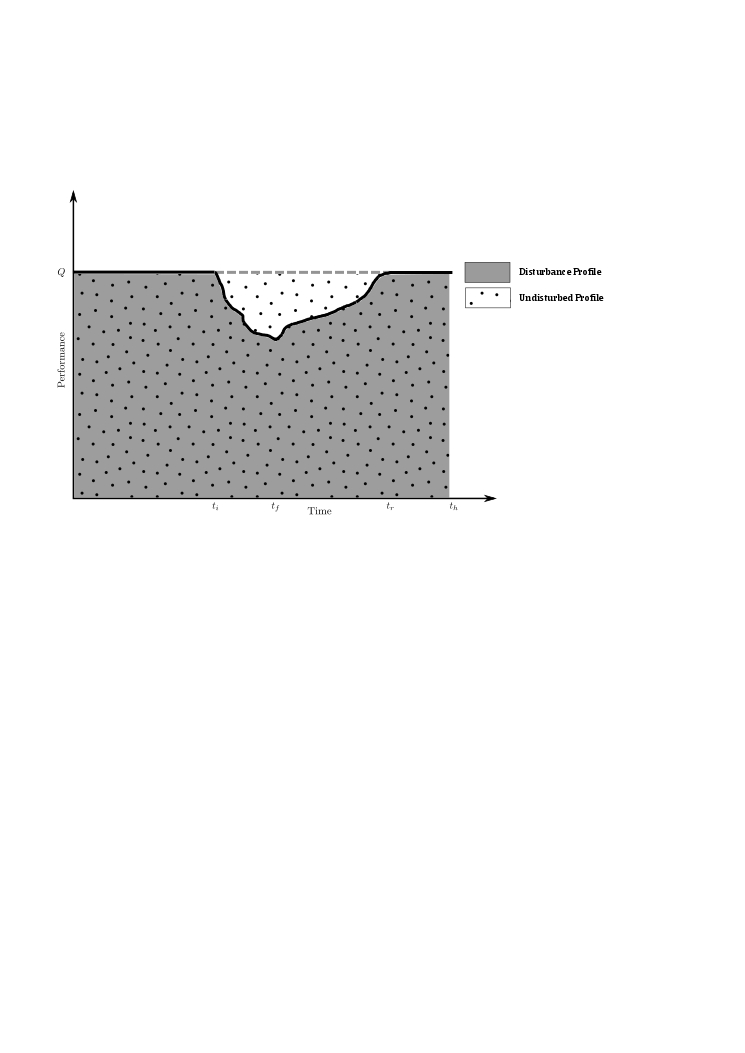
\includegraphics{ResilienceDepiction2}
%  \label{fig:RDpng}
%\end{figure}



\subsection{Robustness}
Robustness is the ``\ldots strenght, or the ability of elements,
systems, and other units of analysis to withstand a given level of
stress or demand without suffering degradation or loss of function.''
Robustness is composed of several different components including
reliability, failure severity, and strength to resist
stressors \cite{Bruneau2003}.

Reliability is a key component of robustness. Reliability is the
``\ldots \emph{ability} of an item \ldots to operate under designated
operating conditions for a designated period of time or number of
cycles.'' \cite{Modarres2010}. A component's reliability is associated with operation
within the intended operating environment. Also, reliability typically
deals systems that are binary. The system is either in a ``working''
status or a ``failed'' status. Resilience accomodates levels of
performance. Thus, reliability is a subset
 of resilience since resilience must account for deviations from the
 intended operating environment. Figure~\ref{fig:Reliability} shows
 the binary behavior of a component's robustness when considering 
 reliability \cite{Ayyub2014c, Modarres2010, Rausand2004}.
 Figure~\ref{fig:Overstress} shows the performance
 profile of the system in the case of overstress assuming a total
 instantaneous failure. Figure~\ref{fig:Reliability} and
 Figure~\ref{fig:Overstress} are visually similar, but conceptually
 different. The overstress marked in Figure~\ref{fig:Overstress}
 represents a departure from the intended operating environment.

\begin{figure}
 \centering
 \includegraphics{Reliability}
 \label{fig:Reliability}
 \caption{Performance in the Case of Reliability}
\end{figure}
 
\begin{figure}
  \centering
  \includegraphics{Overstress}
  \label{fig:Overstress}
  \caption{Performance in the Case of Overstress}
\end{figure}

Another way to improve robustness is to make the failure profile more
graceful. This profile could take any path to the maximum performance
degradation. For illustrative purposes,
Figure~\ref{fig:MultiLevelFailure} shows how a system resisting
complete failure over time adds to the resilience of the system. 

\begin{figure}
  \centering
  \includegraphics{MultiLevelFailure}
  \label{fig:MultiLevelFailure}
  \caption{Improving Robustness through Multi-Level Failure}
\end{figure}

\begin{figure}
  \centering
  \includegraphics{ImprovingReliability23}
  \label{fig:ImpRel23}
  \caption{Improving Robustness through Lengthening Time to Failure}
\end{figure}



\begin{figure}
  \centering
  \includegraphics{strengthStress}
  \label{fig:strengthStress}
  \caption{Improving the Strength of a Component}
\end{figure}



  
